\documentclass{scrartcl}

\usepackage[hidelinks]{hyperref}
\usepackage[none]{hyphenat}
\usepackage{graphicx}
\graphicspath{ {Images/} }

\title{MARKET EVALUATION AND BUSINESS CASE}
\subtitle{COMP240 - Market Evaluation}

\author{JH182233}

\begin{document}
	
	
	\maketitle
\abstract{In modern day gaming it can be difficult to develop a game that stands out from the rest. The case with most games, is that they get lost in the plethora of other games of a similar genre. A method known as “Market research” can help to solve this issue. The main point for market research is to help a developer find a gap in the current market to inform them of design specs that can help them stand out. Though with games it can be difficult to pinpoint the exact gap, a developer can at least get an idea of the state of the market they want to enter is current in. Once this gap has been found, the next step is to find the targeted audience, usually this answer is formed from the gap in the market, but it helps to specifically define the audience so the developer can have some understanding of the impact the game may have.}
	
\section{Method}
For MONQ we have taken the approach described above, find the gap then define the audience. 
\newline

\quad 1:Searching the current market to identify game concepts that have not been  seen or done in some time.

\quad 2:Then finding out if that concept does well in the market, by finding sales  figures and critical reviews, Note: Try to filter the mega fans and trolls,  as they can be bais.  

\quad 3:Once this is done we can try to define our desired audience, and begin the  design process for the game.

\quad 4:As the design progresses we compare the design to our desired audience to  see if our desired audience remains the same or if we have drifted and need  to redefine our desired audience, while being confined to the market gap.

\quad 5:After the design for the game is complete, we can have a final definition  of the target audience.

\quad 6:Once this is done we can calculate the price for the game and begin our  budgeting process.

\quad 7:As the game is developed we must continue to monitor the market to ensure the gap is not filled, if this were the case we may have to redesign the game to fit another gap or abandon the project to start anew. 
\section{Market}
\begin{center}
	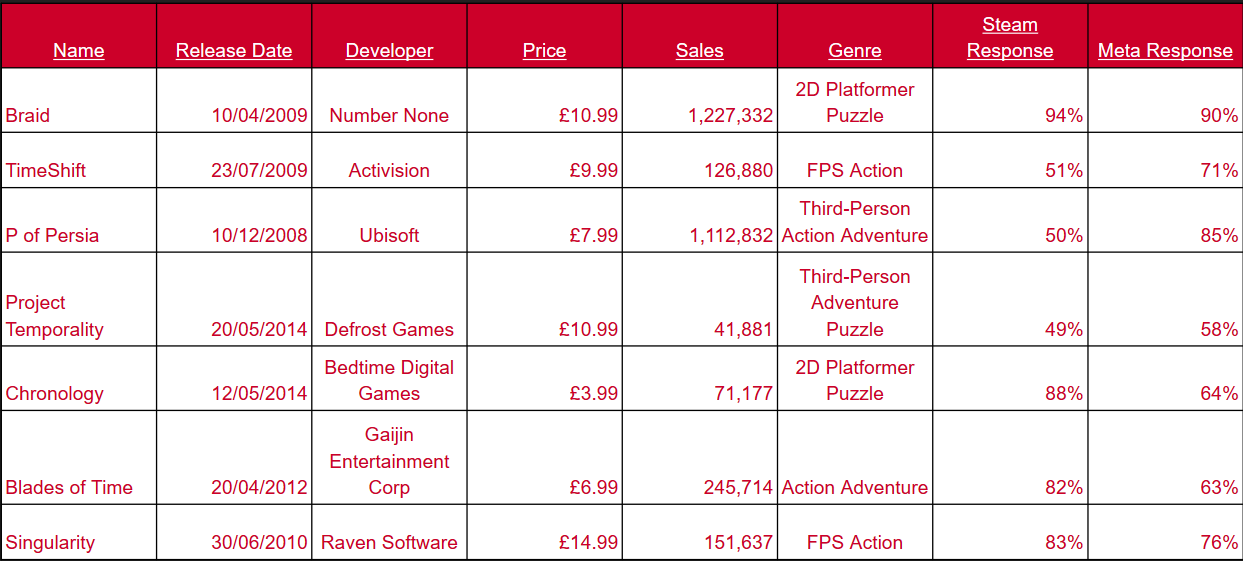
\includegraphics[scale=0.4]{ResearchChart}	
	\newline
\end{center}


The market that was looked into was for steam as that will be our primary sales platform.
Steam currently is selling 13,621 games according to SteamSpy
Looking at Time Manipulation (TM) as a mechanic only 22 are on steam and of those, Seven games where found that match MONQ.
This indicates either a small market for this type of game or a large gap in the market.
From the table there are a mixture of Indie and AAA developers that make TM games.
These games vary from 2D and 3D style games, though the highest sales achieved came from an indie company for a 2D game (Braid).
From the reviews it would seem that the 2D games tend to be received better overall than the 3D games, though the reviews are mixed so this can not carry too much weight.
Looking at the sales, TM games sell well and are considered a success on steam, ranging from £3.99-£14.99.
The last similar game to be released was back in 2014, which would indicate a current gap for TM type games.
After looking at the current market it seems to indicate that the audience we should aim for are not hardcore gamers with high end computers, but gamers that take a more relaxed approach to gaming and enjoy the puzzle element, as most of the games here share the puzzle aspect.
\newline
\newline
\newline
\newline	
When marketing you have to look at two options:
\begin{center}
	Quality of branding
	\newline
	Quantity of reach
	\newline
\end{center}
When looking at quality of branding it can be expensive as you have to go through an agency or higher a marketing specialist.
When looking at quantity of reach you can save money by going through platforms like Social media, which will get you a wide reach but:
You have to ensure the quality and delivery 
Which can lead to a negative effect on your product if done poorly.
Which you may or may not recover from.
Currently Social Media is our main focus for marketing spending a fixed budget on reaching new potential customers.

We plan on marketing through a marketing agency in the near future.
Though more research into which marketing agency will be used there are plenty of agencies in and around Cornwall.
We are primarily using steam as a selling platform as this seems to be one of the biggest platforms for small Indie companies to sell on.
Though we will be launching on itch.io for early access, to access feedback from players on how the game could be improved.
We will be offering our game from our website, but the sales on there are projected to be far less than steam, as currently the traffic through our website is not high enough.

\newpage
\section{Budgets}

The following charts show the monthly costs and income for the next year of production.
\newline
\begin{center}
	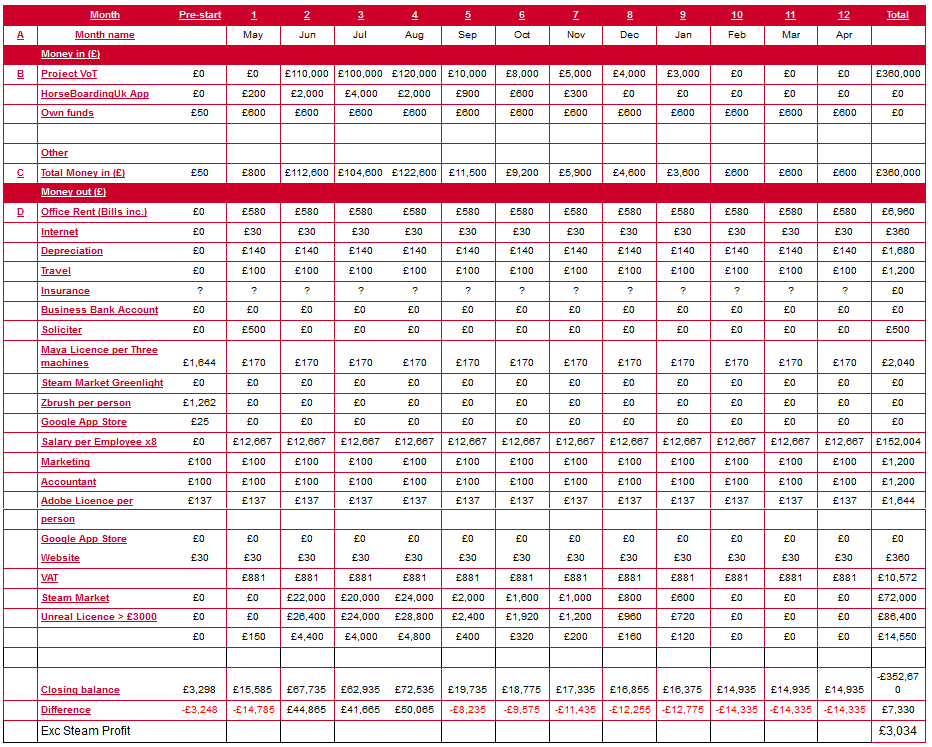
\includegraphics[scale=0.56]{CostsChart}	
	\newline
\end{center}

As you can see we must sell 33,000 units to break even. This is still lower than the worst selling game of similar mechanics on steam.
From play-testing it has been suggested to us that we sell the game for no less than Ten Pounds per copy, this is the price that will be asked for on the marketplace.
\newline
\begin{center}
	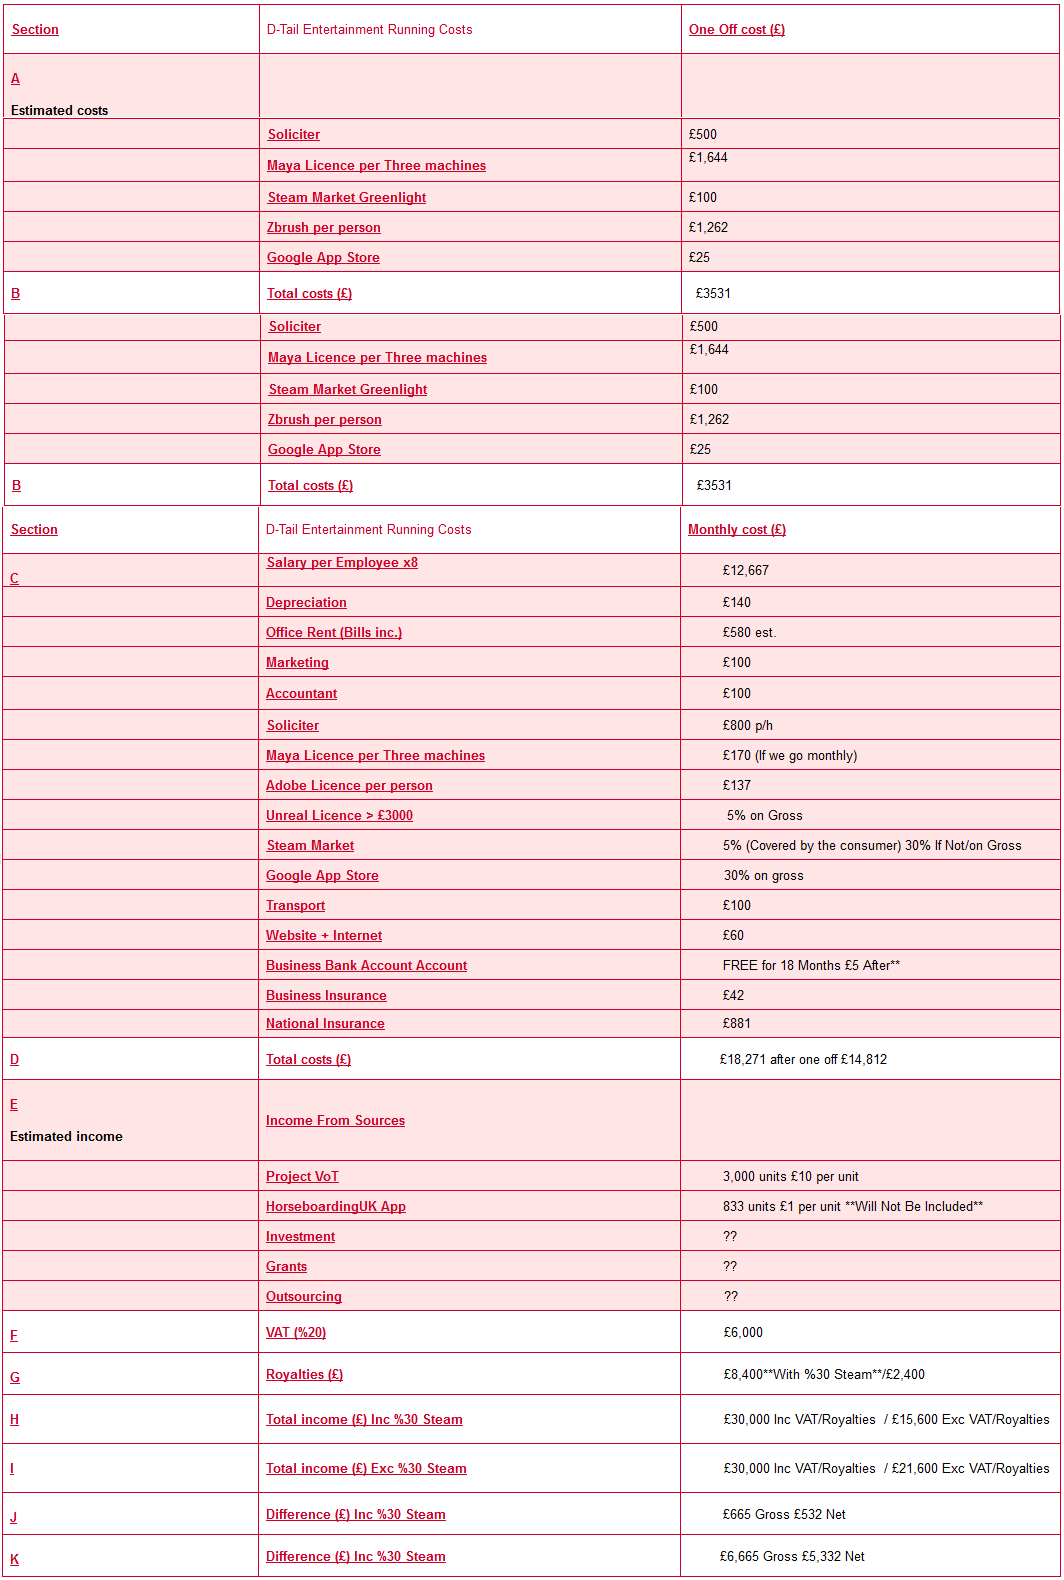
\includegraphics[scale=0.56]{CostsChartLong}
\end{center}
	
											
	\bibliographystyle{apalike}
	\bibliography{Journal}
											
\end{document}